The name of the last prototype, which has been developed in Valencia in the framework of tritium project, is Tritium-IFIC 2. In this prototype, which is showed in the figure \ref{fig:Tritium_IFIC_2}, we have increased the number of fibers used up to 800 which are read out by the same PMTs that we used in the previous experiences. Furthermore, these fibers won't be fixed to a hole matrix like Tritium-IFIC 1 because it is difficult with 800 fibers. In this prototype fibers will be free with they have enough freedom in order to allow the flow of the water through them. 

With this prototype we try to solve the problem that we had with Tritium-IFIC 1 related to the coincidence. 

This prototype is expected to be the last one from which we will build our final detector so, although the water won't flow through this laboratory prototype, it has some modifications in order to be prepared with requirements enough to do so. For example, the internal volume will be circular instead of square like the previous prototype as yo can see in the figure \ref{fig:Tritium_IFIC_2_b}. The reason of that is because, although we would like to keep the internal volume square because the active area of the photosensors is square, a circular internal volume is necessary to facilitate the flow of water. The diameter of this circular volume will be enough large to adjust the square active area of the photosensors inside. Due to that, we will have some scintillating fibers which we don't read, at least directly, but it won't be a problem because it is a cheap material. We will only read, at least directly, more than 500 out of 800 fibers.

\begin{figure}[htbp]
\centering
\subfigure[\label{fig:Tritium_IFIC_2_a}]{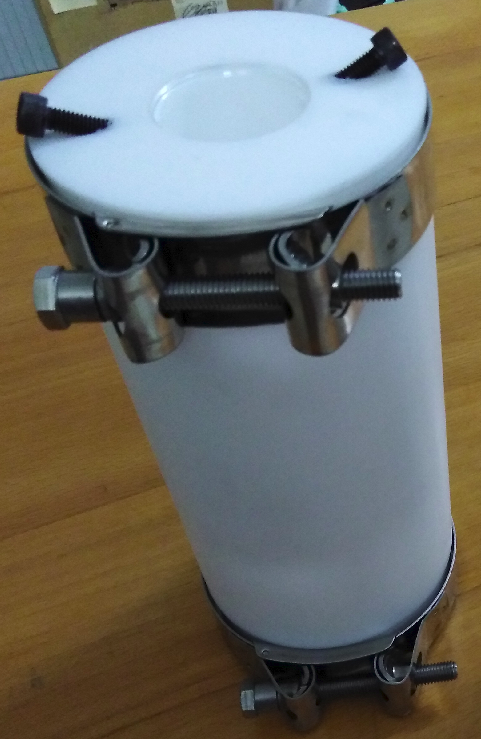
\includegraphics[width=70mm]{./Figuras/Tritium_IFIC_2.png}}
\subfigure[\label{fig:Tritium_IFIC_2_b}]{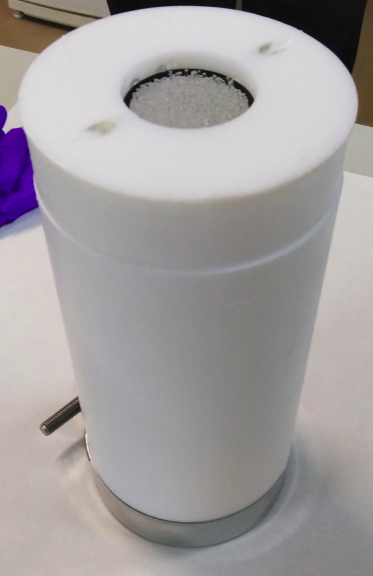
\includegraphics[width=70mm]{./Figuras/Tritium_IFIC_2_2.png}}
\caption{Tritium-IFIC 2 prototype} \label{fig:Tritium_IFIC_2}
\end{figure}

In our last prototypes we have read the fibers directly because in all cases it was on top of the detector. However, it is impossible with this prototype because, as we have seen in our last experiences, we need to keep the fibers straight and read them from both sides so we cannot put both fiber sides on the top of the detector. If the fibers is read on directly, the tritium solution could leak from the side of the fiber that is not on top. 

Therefore, in this prototype, we need a totally closed container inside of which we have the fibers and the tritium solution, whose internal volume is $0.082~\liter$. This container is filled from two holes at the top of the prototype and it has two windows to read the fibers, as you can see in figure \ref{fig:Tritium_IFIC_2}, one at the top of the prototype and one at the bottom. The material of these windows will be PMMA (polymethyl methacrylate) because the light transmission in this material is close to $100\%$ so we don't loss photons and, by extensions, it don't affect to the efficiency of our detector.

Finally a aluminium structure was built for hold several prototypes like it. This structure is shown in the figure \ref{fig:Tritium_IFIC_2_holder}.

\begin{figure}[htbp]
\centering
\subfigure[\label{fig:Tritium_IFIC_2_holder_a}]{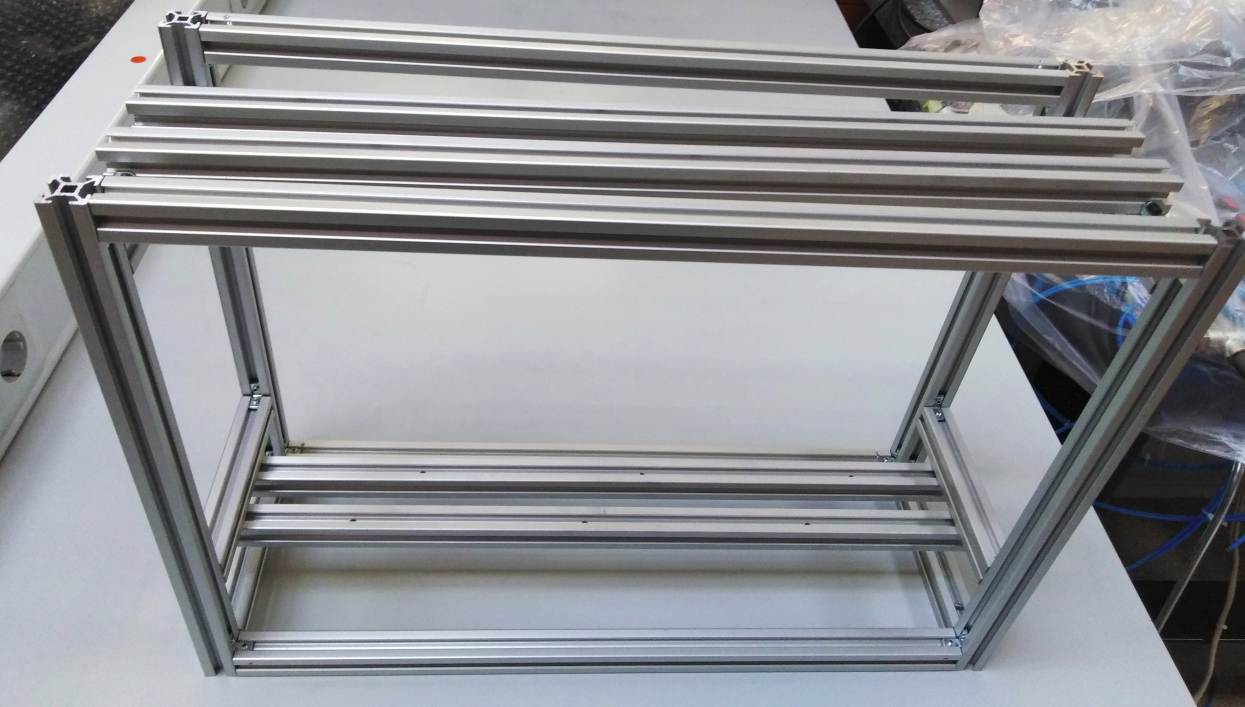
\includegraphics[width=70mm]{./Figuras/Tritium_IFIC_2_Holder.png}}
\subfigure[\label{fig:Tritium_IFIC_2_holder_b}]{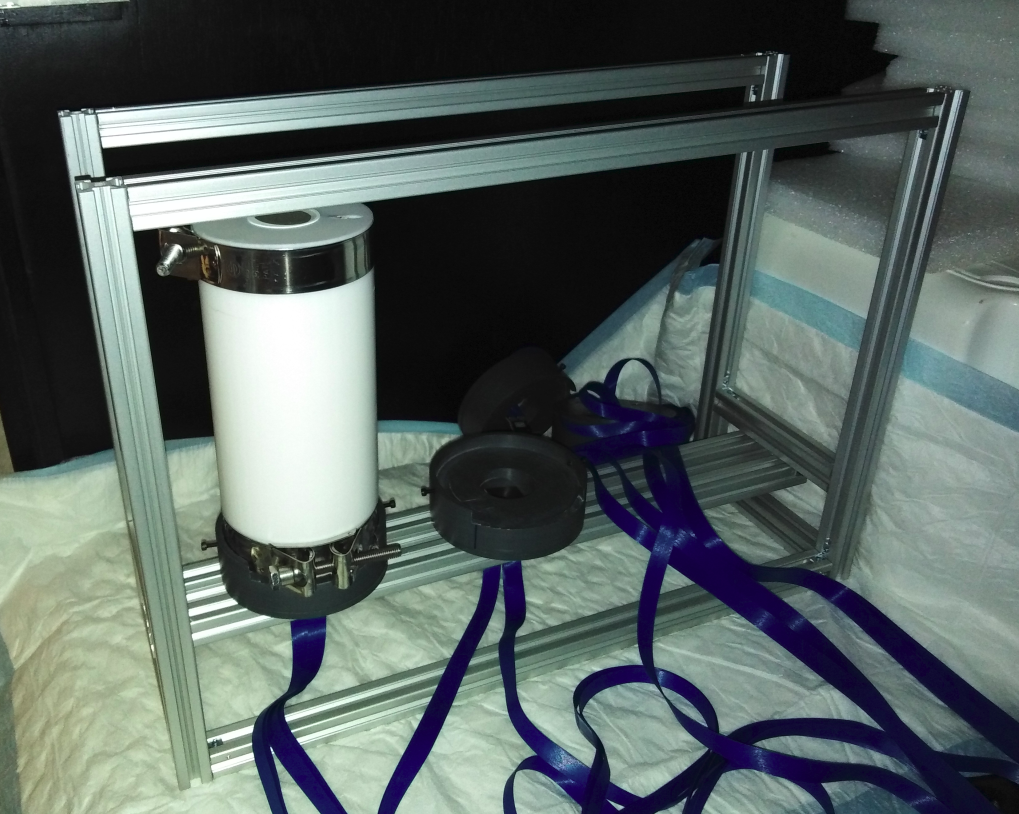
\includegraphics[width=70mm]{./Figuras/Tritium_IFIC_2_Holder_2.png}}
\caption{Tritium-IFIC 2 prototype} \label{fig:Tritium_IFIC_2_holder}
\end{figure}

Similarly like past experiences, the measurements obtained for the background signal and the tritium signal with the same tritium activity are shown in the figure \ref{}:

FIGURAS

CALCULO DE EFICIENCIAS.

In order to check the difference between PMTs and SiPM arrays we repite this experiences but using SiPM arrays as a photosensors. The SiPM arrays used in these experiences are commercial from Hamamatsu, whose serial number is S13361-6075AE-04. It has higher photodetection efficiency, $50\%$ than PMTs, less than $30\%$, so they should get better results. The measurements obtained in this experience is shown in the figure \ref{}

FIGURAS

CALCULA DE EFICIENCIAS

DISCUSIÓN DE CUAL ES MEJOR.
